Having explored both Memcached and Redis, we now turn our attention to a `head to tail' comparison of the object caches. Initially, we focus on a comparison of the default performance. Subsequently, we expand the scope to multiple threads as well as multiple processes.


\section{Out of the Box}

Firstly, let us evaluate the default performance of Memcached and Redis (M\&R). The default performance is an important benchmark as well as a baseline. It is likely that M\&R users who simply require a cache which is `good' enough - performs to expectations, however, scalability is not a concern - will spend less time optimizing the cache performance and tuning the stack.

At this point, it is important to note that Memcached is a multi-threaded application with 4 threads by default. Figure \ref{fig:mr_default} plots M\&R performance with default configuration.

\begin{figure}[h]
    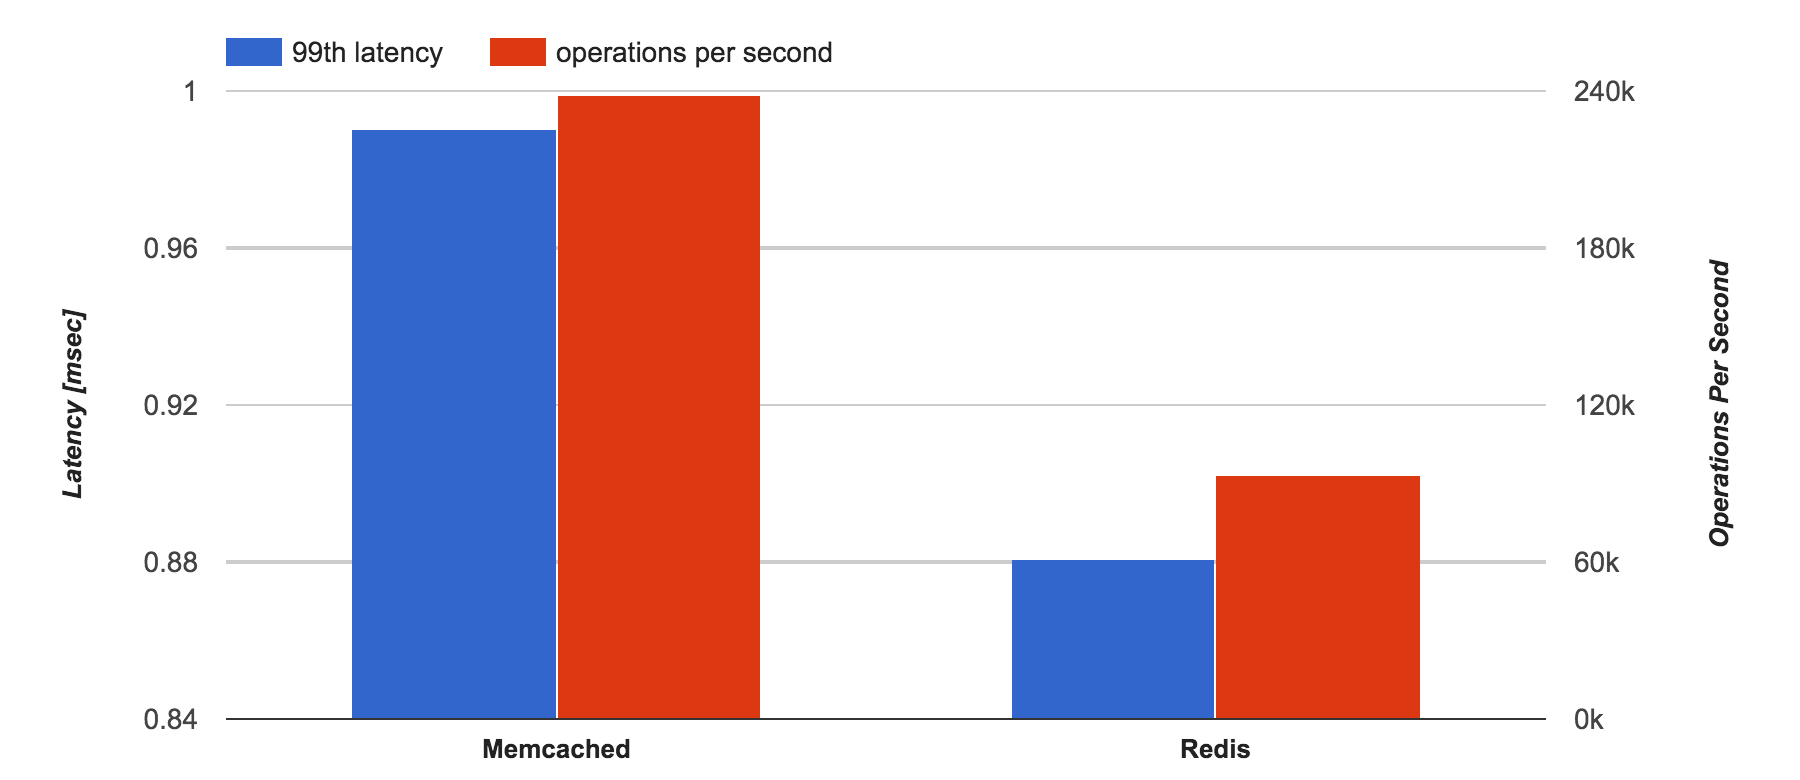
\includegraphics[width=\textwidth]{./res2/mr_default.png}
    \caption{Out of the Box config: 99th percentile latency \& Operations per second}
    \label{fig:mr_default}
\end{figure}

Memcached performs better in its default configuration. This is not an unsurprising result provided Memcached runs with 4 threads while Redis is single threaded. Interestingly, we would expect the performance of Memcached to be on the order of 4 times as much as Redis, however, Memcached only achieves close to 240k requests per second while Redis achieves 93k requests per second. This is about 2.5 times less than Memcached.

With default configuration, Memcached outperforms Redis. This is simply the result of utilizing 4 threads with Memcached. However, in the default configuration Memcached suffers from scalability inefficiencies. A comparison of a 4 threaded application vs a single threaded application may seem unfair, however, it is important to understand the baseline performance. In subsequent sections, we will focus on comparisons on a more even ground.

\section{Scaling Up}
Let us now consider Memcached with multiple threads in comparison to multiple Redis instances. Both M\&R use the same benchmark configuration.

\begin{figure}[h]
    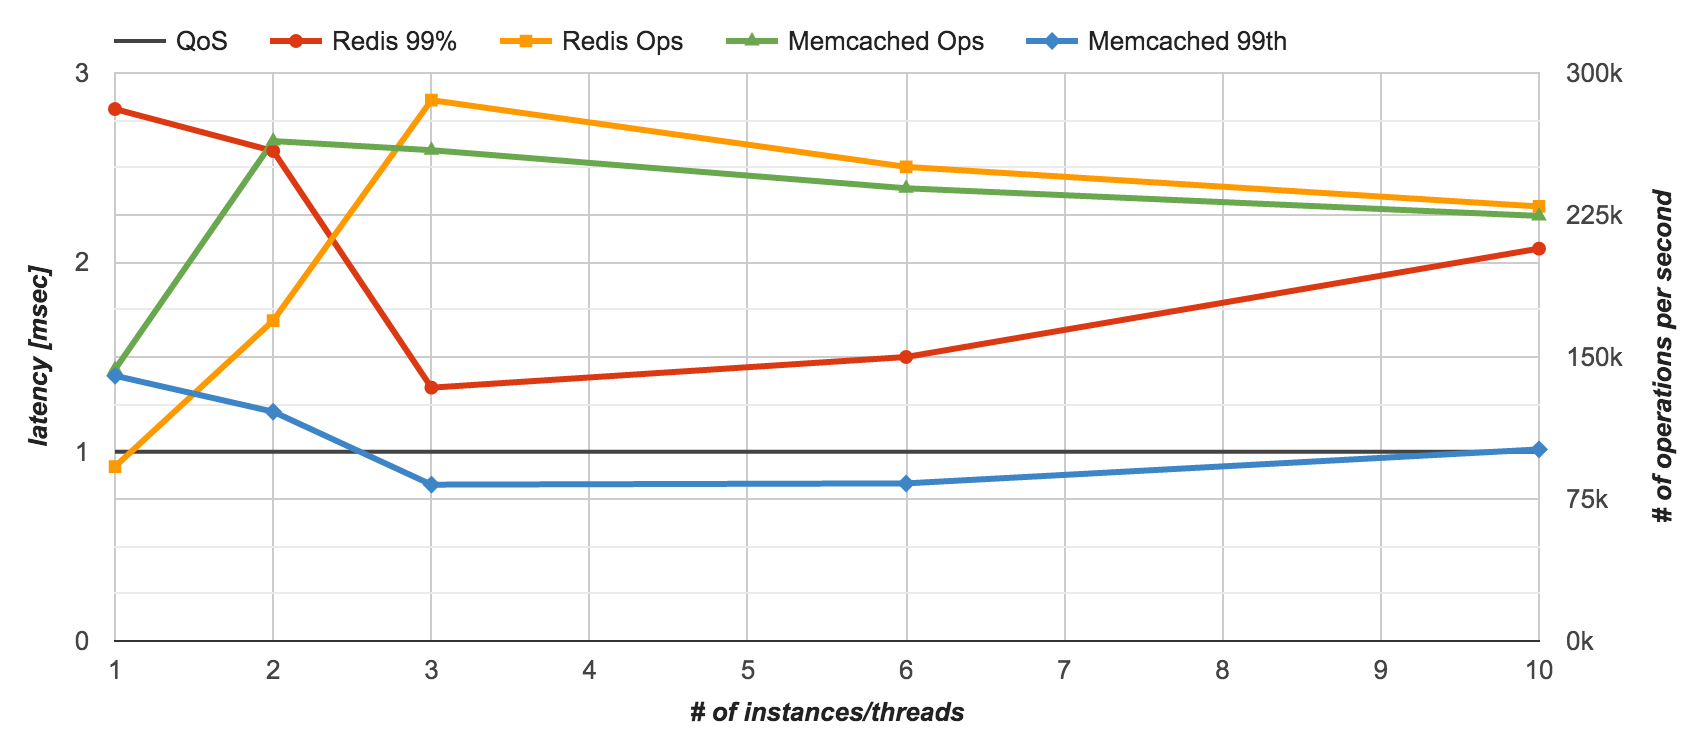
\includegraphics[width=\textwidth]{./res2/mr_instances.png}
    \caption{Memcached Threads vs Redis Instances: 99th percentile latency \& Operations per second}
    \label{fig:mr_instances}
\end{figure}

Figure \ref{fig:mr_instances} plots 99th percentile latency and number of operations per second for both M\&R. Memcached clearly performs better, achieving below QoS 99th percentile latency with a minimum of 0.82 milliseconds at 3 threads. Redis, on the other hand achieves a minimum of 1.33 milliseconds at 3 threads and does not satisfy the QoS. Interestingly, both M\&R reach their respective minimums at 3 threads or instances respectively.

Memcached throughput is maximized at 2 threads with 264k requests per second. Redis throughput, on the other hand, is maximized at 3 threads with 285k requests per second.

\begin{figure}[h]
    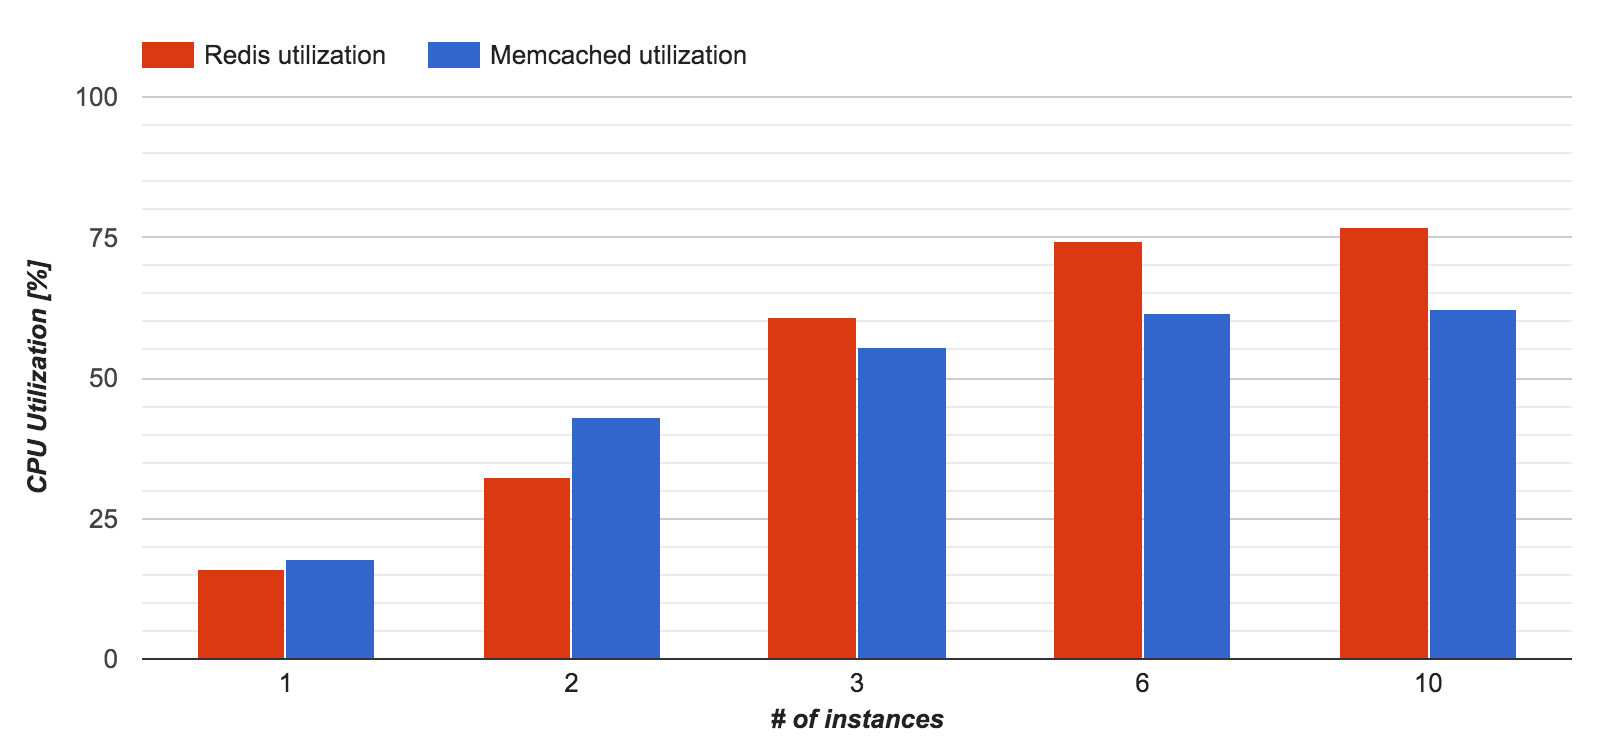
\includegraphics[width=\textwidth]{./res2/mr_instances_cpu.png}
    \caption{Memcached Threads vs Redis Instances: CPU Utilization}
    \label{fig:mr_instances_cpu}
\end{figure}

Figure \ref{fig:mr_instances_cpu} shows CPU utilization against instances. We can observe that at no point do we reach 100\% utilization. This is indicative of the load balance problem explored in previous sections. Additionally, with 1 or 2 threads/instances, Memcached achieves higher CPU utilization than Redis, however, with 3 or more instances, Redis achieves better CPU utilization.

In this direct comparison, Memcached performs better as it actually achieves the desired QoS. However, both caches suffer from load imbalance - software interrupt processing only occurs on a single CPU core which makes it a bottleneck.


\section{Scaling Up with IRQ Pinning}
We have seen in previous chapters that software interrupt processing on a single CPU core greatly decreases overall performance of the cache. In this section, we compare M\&R performance with IRQ pinned.

\begin{figure}[h]
    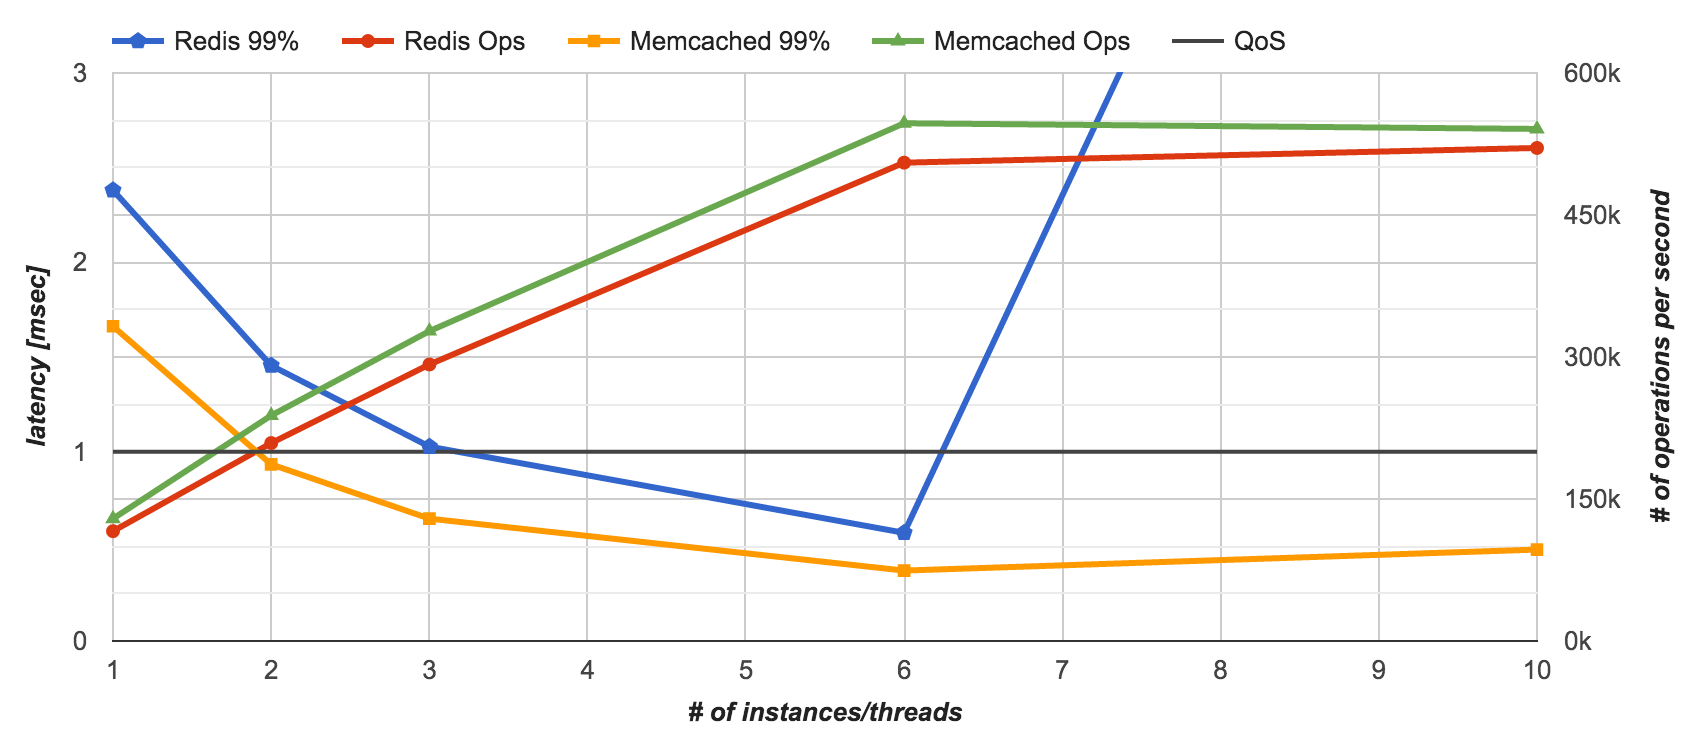
\includegraphics[width=\textwidth]{./res2/mr_irq.png}
    \caption{Memcached Threads vs Redis Instances with IRQ pinned: Latency \% Throughput}
    \label{fig:mr_irq}
\end{figure}

Figure \ref{fig:mr_irq} plots 99th percentile latency and operations per second for both M\&R. Firstly, 99th percentile latency is minimized for both M\&R at 6 threads/instances. Redis reaches a minimum of 0.57 ms while Memcached 99th percentile latency is 0.44 ms. Memcached clearly performs better in terms of 99th percentile at minimum. Additionally, Memcached achieves the desired QoS with 2 or more instances while Redis only achieves the QoS with 6 threads.

Secondly, the number of operations per second within QoS peaks at 6 threads for both M\&R. Memcached achieves 546k operations per second while Redis executes 505k requests per second. Both caches experience a linear growth in throughput up to 6 threads at which point the number of operations flattens out.

\begin{figure}[h]
    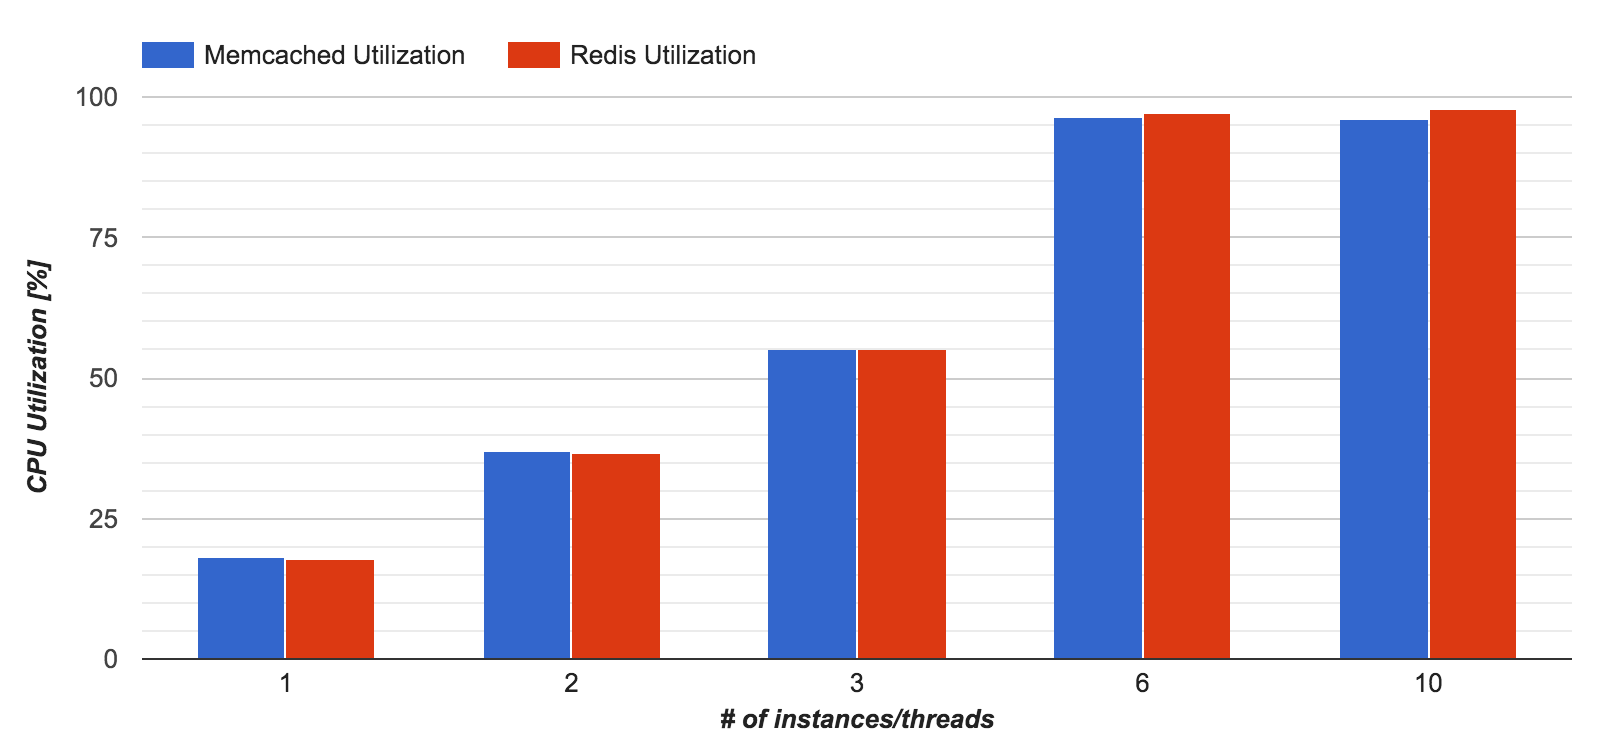
\includegraphics[width=\textwidth]{./res2/mr_irq_cpu.png}
    \caption{Memcached Threads vs Redis Instances with IRQ pinned: CPU Utilization}
    \label{fig:mr_irq_cpu}
\end{figure}

Figure \ref{fig:mr_irq_cpu} plots the CPU utilization against the number of instances/threads. We can observe that CPU utilization increases linearly with the number of instances for M\&R. Additionally, M\&R exhibit the same CPU utilization with a given number of instances. This is unsurprising given similar levels of throughput and latency as well as majority of execution time spent in the kernel and processing software interrupts, we would not expect to see significant differences between the two caches.

In a previous chapter on Memcached, we have also investigated the performance of Memcached when deployed in a multi-instance setup with 1 thread - in effectively single threaded mode. We have found that there is very little difference in performance (\ref{m_instances_latency}). We concluded that a multi-instance Memcached setup with 1 thread performs as good as a single instance multi-threaded setup.

In previous chapters, we have considered additional optimizations such as thread/process pinning or group size in the case Memcached, however, we found that those optimizations did not increase performance further. Therefore,

Overall, we find that Memcached outperforms Redis. Memcached achieves lower 99th percentile latency with higher throughput.

\section{Object Size}

\begin{figure}[h]
    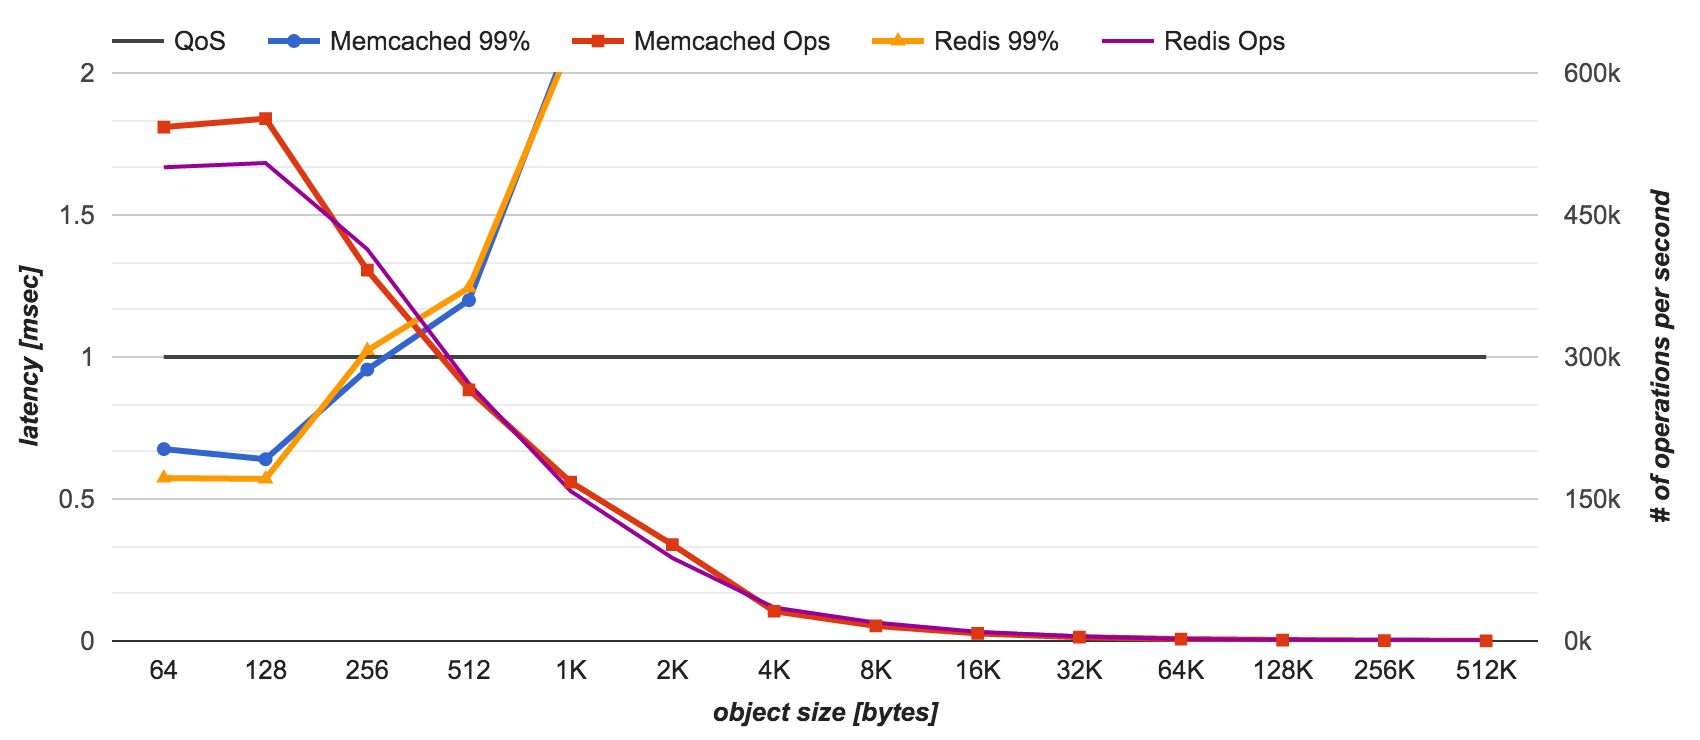
\includegraphics[width=\textwidth]{./res2/mr_object_size.png}
    \caption{Memcached vs Redis: Latency \& Throughput vs Object Size}
    \label{fig:mr_object_size}
\end{figure}

In this comparison, we consider M\&R with respect to object size. Figure \ref{fig:mr_object_size} plots the 99th percentile latency and number of operations per second against object size. We find that both caches scale well up to 128 bytes, however, their performance begins to degrade with object sizes 256 bytes and greater. Memcached satisfies the QoS object size of 256 bytes while Redis exceeds the QoS mark. A further increase in object size leads to decreased number of operations per second and increased 99th percentile latency. The network performance starts to dominate the execution time and the overall performance degrades. This is further apparent from Figure \ref{fig:mr_object_size_cpu}.

\begin{figure}[h]
    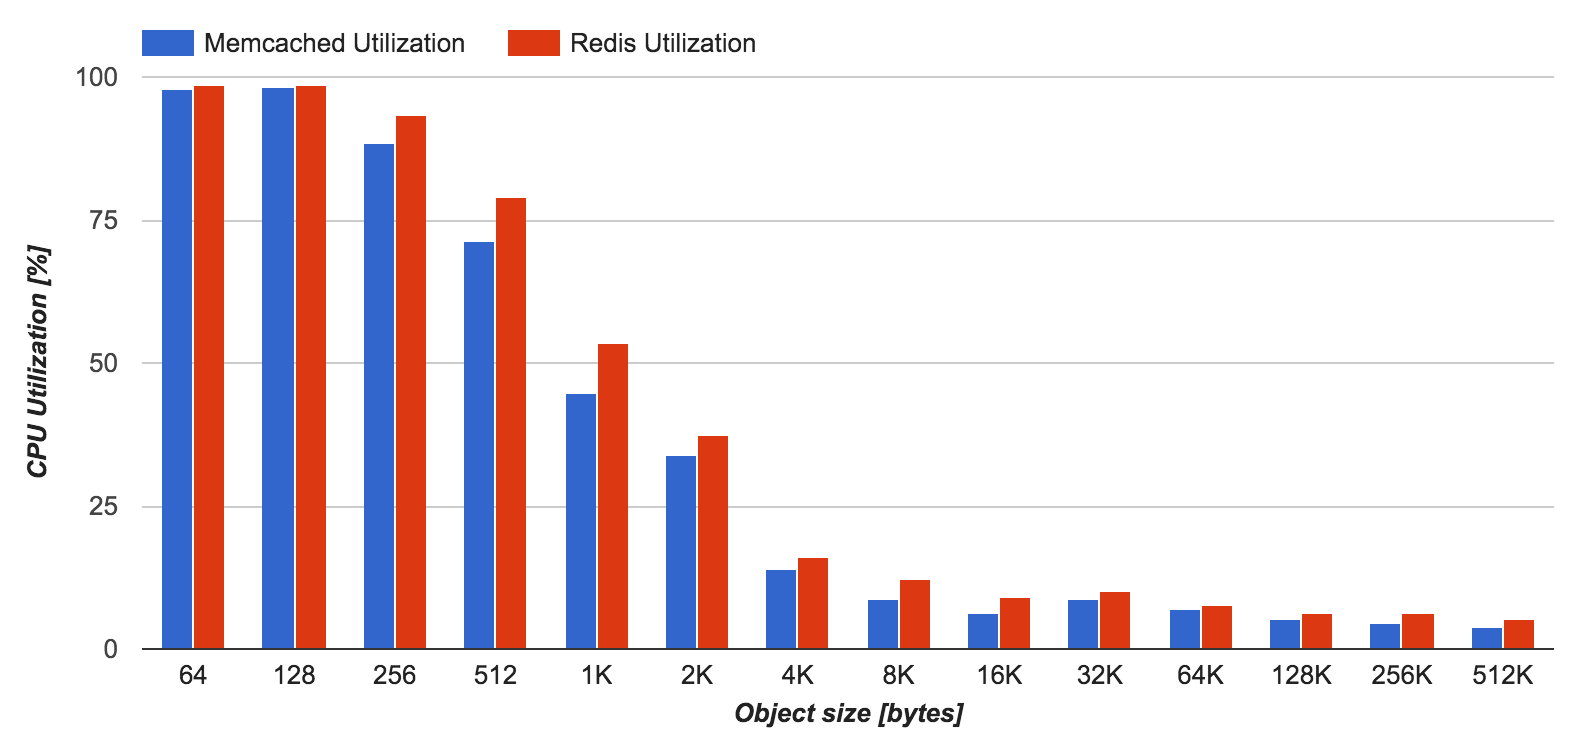
\includegraphics[width=\textwidth]{./res2/mr_object_size_cpu.png}
    \caption{Memcached vs Redis: Latency \& Throughput vs Object Size}
    \label{fig:mr_object_size_cpu}
\end{figure}

As object size increases, we achieve lower server CPU utilization. Furthermore, we can observe that CPU utilization remains similar, with Redis slightly higher than Memcached, between M\&R at various object sizes.

